\section{EC 1.1}

\textbf{Exercise 1.0.1} (Information set). \textit{What is an information set?}\\\\
An information set $h$ of player $i$ is a subset of $ V_{i} $ such that, for all $w, w^{\prime} \in h$ the property $ \rho(w) = \rho(w^{\prime}) $ holds (with an abuse of notation, we denote $ \rho(h)$ as $\rho(w) $ with $w \in h $).\\\\
\textbf{Exercise 1.0.2} (Perfect vs. imperfect information). \textit{Report an example of 2-player game in extensive-form
representation with perfect information and an example of 2-player game with imperfect information.}
\begin{figure}[H]
\begin{subfigure}[t]{0.45\textwidth}
 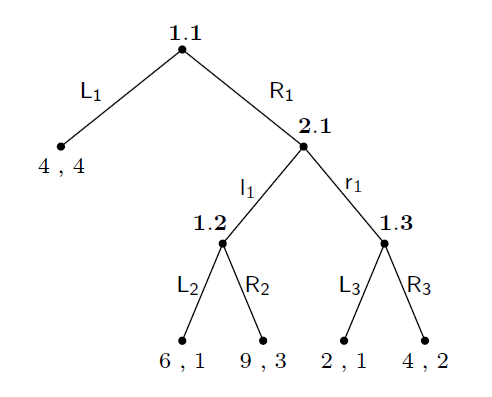
\includegraphics[width=\textwidth]{images/img_1_1_01.png}
 \caption{With perfect information}
\end{subfigure}
\begin{subfigure}[t]{0.45\textwidth}
 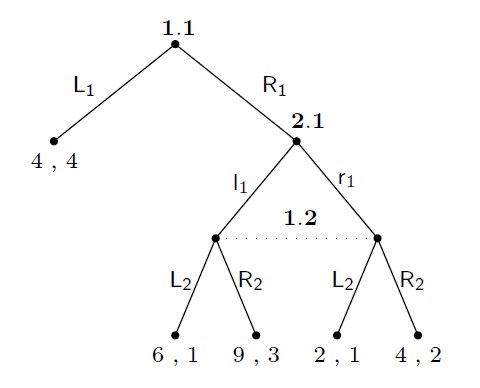
\includegraphics[width=\textwidth]{images/img_1_1_02.png}
 \caption{Without perfect information}
\end{subfigure}
\end{figure}
\noindent
\textbf{Exercise 1.0.3} (Perfect recall). \textit{Report the definition of perfect-recall games in terms of constraints over the
information sets of the players.}\\\\
Player $i$ has perfect recall in an imperfect-information extensive-form game if for any two decision nodes $ w, w^{\prime} $ that are in the same information set $h$ for player $i$, for any path $ \langle w_{0}, a_{0}, w_{1}, a_{1}, w_{2}, \ldots, w_{k}, a_{k}, w \rangle $ from the root $\bar{w}_{0}$ of the game to $w$ (where $w_{j}$ are decision nodes of player $i$ and $a_{j}$ are actions played at $w_{j}$ by player $i$) and for any path $ \langle w_{0}^{\prime}, a_{0}^{\prime}, w_{1}^{\prime}, a_{1}^{\prime}, w_{2}^{\prime}, \ldots, w_{l}^{\prime}, a_{l}^{\prime}, w^{\prime} \rangle $ from the root of
the game to $ w^{\prime} $ it must be the case that:
\begin{itemize}
\item $ k = l $;
\item for all $ 0 \leqslant j \leqslant k, w_{j} $ and $ w_{j}^{\prime} $ are in the same information set for player $i$;
\item for all $ 0 \leqslant j \leqslant k $, it holds $ a_{j}=a_{j}^{\prime} $;
\end{itemize}
A game is with perfect recall if every player has perfect recall in it.\\\\
\textbf{Exercise 1.0.4} (Perfect vs. imperfect recall). \textit{Report an example of 2-player game in extensive-form representation
with perfect recall and an example of 2-player game with imperfect recall.}
\begin{figure}[H]
\begin{subfigure}[t]{0.45\textwidth}
 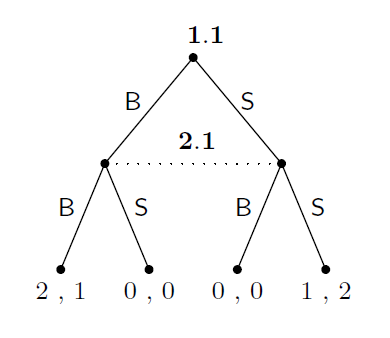
\includegraphics[width=\textwidth]{images/img_1_1_03.png}
 \caption{With perfect recall}
\end{subfigure}
\begin{subfigure}[t]{0.45\textwidth}
 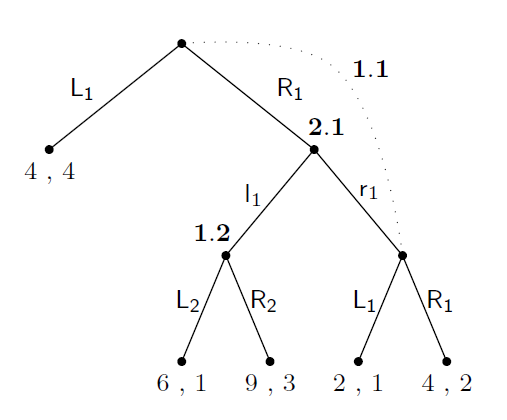
\includegraphics[width=\textwidth]{images/img_1_1_04.png}
 \caption{Without imperfect recall}
\end{subfigure}
\end{figure}
\noindent
\textbf{Exercise 1.0.5} (Timeability). \textit{Report the definition of timeable extensive-form game.}\\\\
Given an extensive-form game, the information sets are chronologically ordered when there is an assignment of labels $l \in \mathbb{N}$ to the decision nodes such that:
\begin{itemize}
\item each decision node has a label strictly larger than the label of the parent;
\item all the decision nodes of the same information set have the same label.
\end{itemize}
The labels have a simple interpretation, being the time at which the information set is traversed.\\
A game is timeable, in the sense that all the players have the sense of time, if and only if all the information sets are chronologically ordered.\\\\
\textbf{Exercise 1.0.6} (Timeable vs. non-timeable). \textit{Report an example of 3-player game in extensive-form representation
with perfect recall in which some player has not the sense of time.}
\begin{figure}[H]
\centering
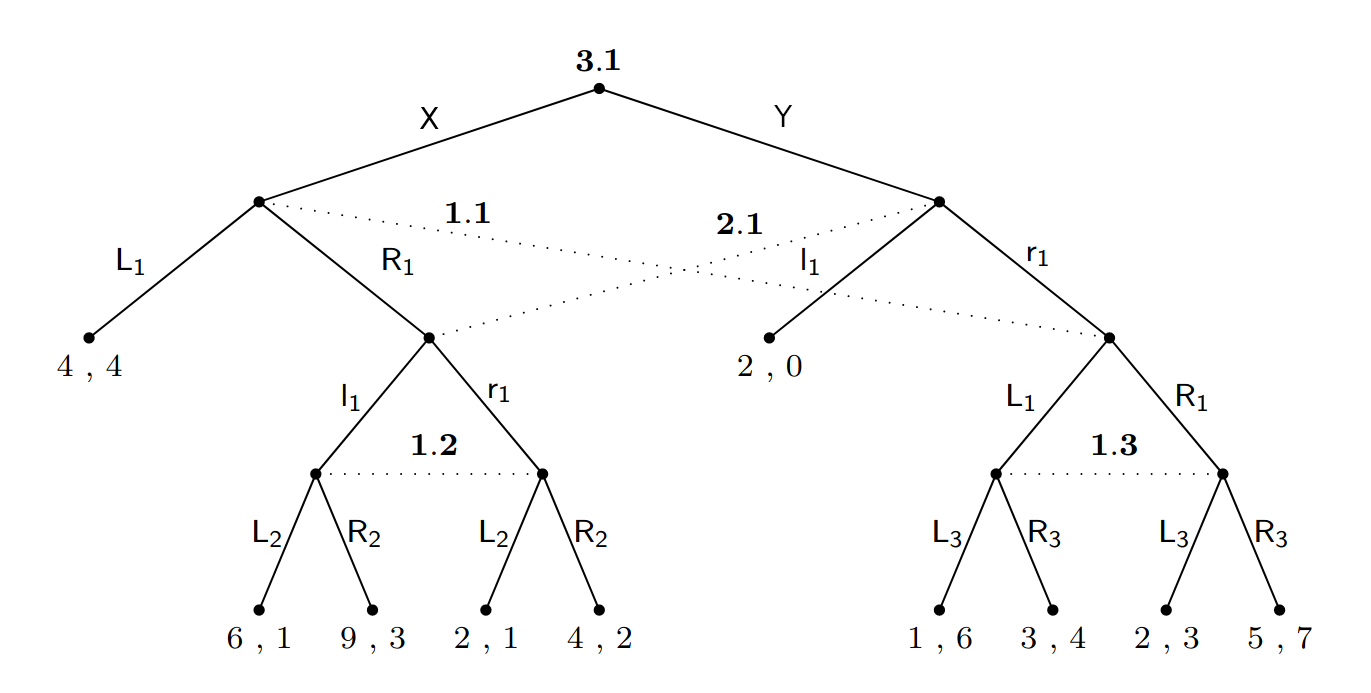
\includegraphics[width=\textwidth]{images/img_1_1_05.png}
\end{figure}
\noindent
\textbf{Exercise 1.0.7} (Game with Nature). \textit{Report an example of 2-player game in extensive-form representation
with Nature.}
\begin{figure}[H]
\centering
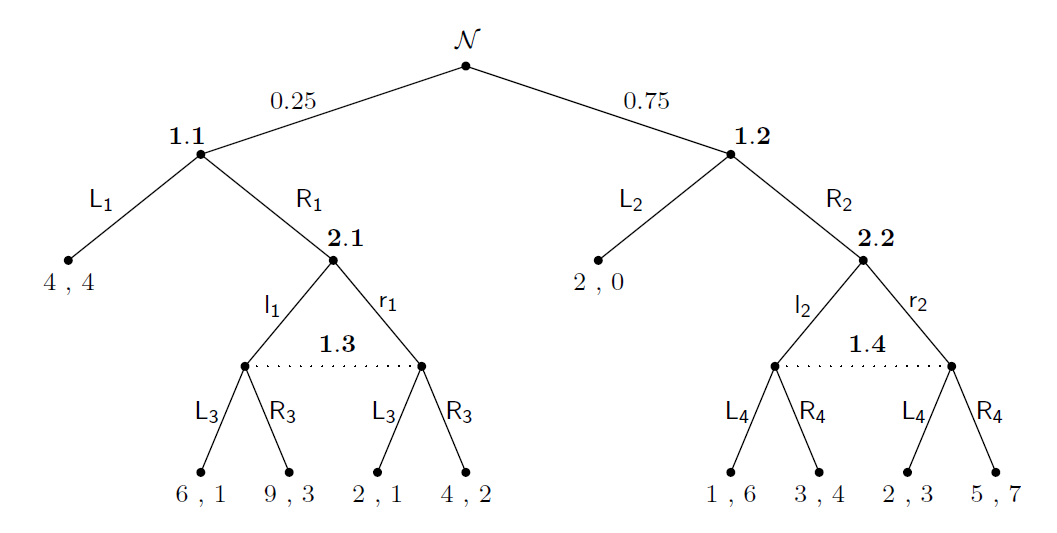
\includegraphics[width=\textwidth]{images/img_1_1_06.png}
\end{figure}
\noindent
\textbf{Exercise 1.0.8} (Kuhn Poker). \textit{Consider the Kuhn Poker game:
\begin{itemize}
\item there are two players \{1, 2\};
\item there are three cards \{K, Q, J\};
\item each player antes 1;
\item each player is dealt one of the three cards, and the third is put aside unseen (no player can observe the
cad of the opponent);
\item player 1 can check or bet 1;
\begin{itemize}
\item if player 1 checks then player 2 can check or bet 1;
\begin{itemize}
\item if player 2 checks there is a showdown for the pot of 2;
\item if player 2 bets then player 1 can fold or call;
\begin{itemize}
\item if player 1 folds then player 2 takes the pot of 3;
\item if player 1 calls there is a showdown for the pot of 4;
\end{itemize}
\end{itemize}
\item if player 1 bets then player 2 can fold or call;
\begin{itemize}
\item if player 2 folds then player 1 takes the pot of 3;
\item if player 2 calls there is a showdown for the pot of 4;
\end{itemize}
\end{itemize}
\item in the showdown, the player with the highest card wins the pot entirely.
\end{itemize}
Provide the extensive-form representation of the game.}
\begin{figure}[H]
\centering
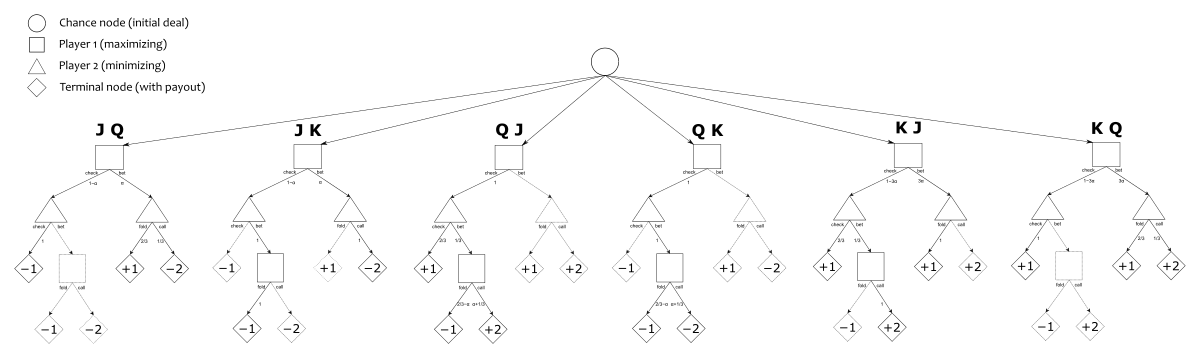
\includegraphics[width=\textwidth]{images/img_1_1_07.png}
\end{figure}
\noindent
\textbf{Exercise 1.0.9} (Simplified bargaining game). \textit{Consider the following simplified bargaining game:
\begin{itemize}
\item there are two players, one buyer b and one seller s;
\item the seller player is of two types: $ \theta_{s.1} $ with a probability of 0.33 and $ \theta_{s.2} $ with a probability of 0.67;
\item the first player can offer either 0.33 or 0.66 and the action is perfectly observable;
\item the second player can accept the offer x of the first player, counteroffer $ x \pm 0.20 $, and this action is
perfectly observable;
\begin{itemize}
\item if the second player counteroffers, then the first player can accept the offer x of the second player,
counteroffer $ x \pm 0.10 $, and this action is perfectly observable;
\begin{itemize}
\item if the first player counteroffers, then the second player can accept or reject;
\begin{itemize}
\item if the second player accepts, the game concludes with an agreement over the last offer
x;
\item if the second player rejects, the game concludes with a disagreement;
\end{itemize}
\item if the first player accepts, the game concludes with an agreement over the last offer x;
\end{itemize}
\item if the second player accepts, then the game concludes with an agreement over the last offer x;
\end{itemize}
\item the utility of all the players from a disagreement is 0, while the utility of buyer from an agreement (x, t)
where t is the time at which the agreement is achieved, is $ (1-x)(\delta_{b})^{t} $, while the utility of seller s.i is $ (\delta_{s.i})^t $. Assume that $ \delta_{b} = 0.5,  \delta_{s.1} = 0.4, \delta_{s.2} = 0.9 $. Each action requires a unitary temporal cost.
\end{itemize}
Provide the extensive-form representation of the game in both cases the first player is the seller (and the second is the buyer) and the first player is the buyer (and the second is he seller).}\\\\
\textcolor{red}{TODO}\\\\
\textbf{Exercise 1.0.10} (Simplified patrolling game). \textit{Consider the following simplified patrolling game:
\begin{itemize}
\item there are two players, one attacker a and one defender d;
\item there is a fully connected graph with four vertices labeled $ \{v_1, v_2, v_3, v_4\} $;
\item the defender is initially at $ v_1 $ and spends one time point to move from any vertex to any another vertex;
\item at time 1, the attacker decides which vertex to attack among $ \{v_2, v_3, v_4\} $ and moves to it, simultaneously
the defender decides the next vertex to visit among $ \{v_2, v_3, v_4\} $;
\item at time 2, the defender covers the vertex which it got and decides the next vertex to visit among all the
vertices not visited yet;
\item at time 3, the defender covers he vertex which it got;
\item if the defender covers the vertex under attack, then the utility of the defender is 1, while the utility of
the attacker is 0, else the utility of the defender is $ 1 - \pi(v_i) $ where $ v_i $ is the attacked target, while the
utility of the attacker is $ \pi(v_i) $.
\end{itemize} 
Provide the extensive-form representation of the game.}\\\\
\textcolor{red}{TODO}\\\\

\section{EC 1.2}
\textbf{Exercise 2.0.1} (Normal-form representation of an extensive-form game). \textit{Provide the definition of the normal-form
representation of an extensive-form game (even in the case games with Nature).}\\\\
Given an extensive-form game $(N, A, V, T, \iota, \rho, \chi,U,H)$, the corresponding normal-form representation is a triplet $(N, P,U')$, in which:
\begin{itemize}
\item $P = \{P_1, P_2, \ldots , P_n\}$ is the set of actions (said plans) of the players and each plan $p \in P_i$ is a tuple specifying one action $a \in A_i$ per information set $h \in H_i$ of player $i$ such that $a \in \rho(h)$
\item $U' = \{U_1,U_2, \ldots ,U_n\}$ is the set of utility functions of the players with $U_i' : P_1 \times  P_2 \times \ldots  P_n \rightarrow \mathbb{R}$ such that $U_i'(p_1, p_2, \ldots, p_n) = U_i(w)$ where $w$ is the terminal node reached by applying plan profile $(p_1, p_2, \ldots, p_n)$.
\end{itemize}
\textbf{Exercise 2.0.2} (Normal-form size). \textit{Given an extensive-form game with 2 players, h information sets per player and 2 actions available to each player at each information set, what is, in the worst case, the asymptotical size of the normal-form representation in h?}\\\\
The normal-form representation of an extensive-form game may have exponential size in the size of the game tree, where the size of the normal-form representation is $|P_1| |P_2| \ldots |P_n|$ and the size of the game tree is $|T|$. The size of the normal-form representation, in terms of $h$, is $|P_1||P_2| = 2^h \cdot 2^h = 2^{2h}$.\\\\
\textbf{Exercise 2.0.3} (Strategy and strategy profile). \textit{Provide the definition of strategy and strategy profile for a game in normal-form representation.}\\\\
A normal-form strategy $ \sigma_{i}: P_{i} \rightarrow [0,1] $ with $ \sigma_{i} \in \Delta (P_{i}) $ is a function returning the probability with which each plan $ p_{i} \in P_{i} $ is played by player i (we denote with $ \Delta(\cdot) $ the simplex over $ \cdot $ ).\\
Strategy profile $ \bm{\sigma} $ is a tuple $ (\sigma_{1}, \sigma_{2}, \ldots, \sigma_{n}) $, containing one strategy per player. Strategy profile $ \bm{\sigma}_{-i} $ is a tuple $ (\sigma_{1}, \sigma_{2}, \ldots, \sigma_{i-1}, \sigma_{i+1}, \ldots, \sigma_{n} ) $, containing one strategy per player except for player $i$.\\\\
\textbf{Exercise 2.0.4} (Reduced normal-form representation of an extensive-form game). \textit{Provide the definition of
the reduced normal-form representation of an extensive-form game.}\\\\
Given the normal-form representation with plans $ P_{1}, P_{2}, \ldots, P_{n} $ of an extensive-form game, the reduced normal-form representation is composed of a subset of plans $ P_{1}^{\prime}, P_{2}^{\prime}, \ldots, P_{n}^{\prime} $ with $ P_{i}^{\prime} \subseteq P_{i} $ such that:
\begin{itemize}
\item no $ p_{i}, p_{i}^{\prime} \in P_{i}^{\prime} $ with $ p_{i} \neq p_{i}^{\prime} $ are realization equivalent;
\item every $ p_{i} \in P_{i} \backslash P_{i}^{\prime} $ is realization equivalent to some $ p_{i}^{\prime} \in P_{i}^{\prime} $
\end{itemize}
\textbf{Exercise 2.0.5} (Reduced normal-form size). \textit{Given an extensive-form game with 2 players, h information
sets per player and 2 actions available to each player at each information set, what is, in the worst case, the
asymptotical size of the reduced normal-form representation in h?}\\\\
The reduced normal-form representation of an extensive-form game may have exponential size in the size of the game tree, where the size of the normal-form representation is $|P'_1| |P'_2| \ldots |P'_n|$ and the size of the game tree is $|T|$. The size of the normal-form representation, in terms of $h$, is $|P'_1||P'_2| = 2^h \cdot 2^h = 2^{2h}$.\\\\
\textbf{Exercise 2.0.6} (Translation). \textit{Given an extensive-form game (even with Nature), provide the corresponding normal-form representation and the corresponding reduced normal-form representation.}
\begin{figure}[H]
\begin{subfigure}[t]{0.3\textwidth}
 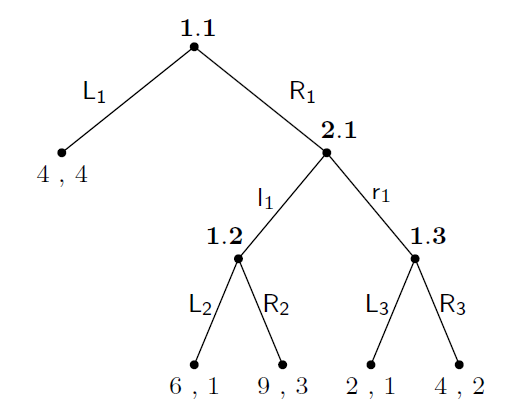
\includegraphics[width=\textwidth]{images/img_1_2_01.png}
 \caption{Extensive-form}
\end{subfigure}\hfill
\begin{subfigure}[t]{0.3\textwidth}
 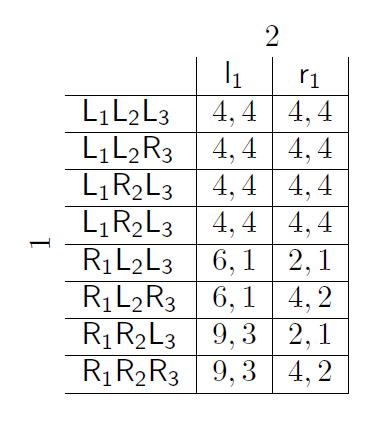
\includegraphics[width=\textwidth]{images/img_1_2_02.png}
 \caption{Normal-form}
\end{subfigure}\hfill
\begin{subfigure}[t]{0.3\textwidth}
 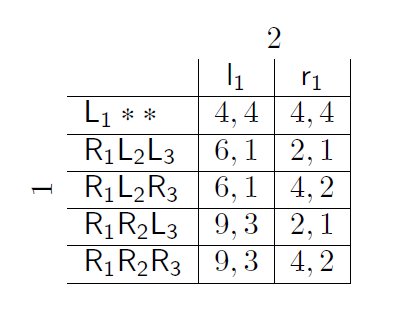
\includegraphics[width=\textwidth]{images/img_1_2_03.png}
 \caption{Reduced normal-form}
\end{subfigure}
\end{figure}
\noindent
\textbf{Exercise 2.0.7} (Expected utility). \textit{Given a game in normal-form with n players, provide the formula of the
expected utility for a player i.}\\\\
Expected utility $ \mathbb{E}_{\mathbf{a} \sim \bm{\sigma}} [U_{i(\mathbf{a})}] $ returns the expected value of the utility of player $i$ given strategy profile $ \bm{\sigma} $. The formula $ \mathbb{E}_{\mathbf{a} \sim \bm{\sigma}} [U_{i}(\mathbf{a})] $ can be written as:
$$
\mathbb{E}_{\mathbf{a} \sim \bm{\sigma}} [U_{i}(\mathbf{a})] = 
\sum_{a_{1} \in A_{1}} \sum_{a_{2} \in A_{2}} \ldots \sum_{a_{n} \in A_{n}}
\sigma_{1}(a_{1}) \sigma_{2}(a_{2}) \ldots \sigma_{n}(a_{n})
U_{i}(a_{1}, a_{2}, \ldots, a_{n})
$$
The degree of the polynomial is $ n $ and, given player $ i $, the expected utility is linear in player \textit{i}'s strategy.\\\\

\section{EC 1.4}
\textbf{Exercise 4.0.1} (Sequence-form representation of an extensive-form game). \textit{Provide the definition of the sequence-form representation of an extensive-form game (even in the case games with Nature).}\\\\
Given an extensive-form game $(N, A, V, T, \iota, \rho, \chi, U, H)$,  the corresponding sequence-form representation is a tuple $ (N, Q, U^{\prime}, C) $,  where:
\begin{itemize}
\item $N$ is the set of agents;
\item $ Q=\left\{Q_{1}, Q_{2}, \ldots, Q_{n}\right\}$ is the set of sequences of all the players and $Q_{i}$ is the set of sequences of player $i$
\item $U^{\prime}=\left\{U_{1}^{\prime}, U_{2}^{\prime}, \ldots, U_{n}^{\prime}\right\}$ is the set of utility functions of all the players where $U_{i}^{\prime}: Q_{1} \times Q_{2} \times \ldots \times Q_{n} \rightarrow \mathbb{R}$ returns the utility $U_{i}(w)$ of the terminal node $w$ reached by a profile of terminal sequences, while it is not defined if the profile of sequences contains at least a non-terminal sequence;
\item $ C=\left\{\left(F_{1}, f_{1}\right),\left(F_{2}, f_{2}\right), \ldots,\left(F_{n}, f_{n}\right)\right\}$ is the set of the constraints over the sequence-form strategies of all the players.\\\\
\end{itemize}
\textbf{Exercise 4.0.2} (Sequence-form size). \textit{Given an extensive-form game with 2 players, h information sets per player and 2 actions available to each player at each information set, what is, in the worst case, the asymptotical size of the sequence-form representation in h?}\\\\
The sequence-form representation has a size linear in the size of the game tree, containing a number of sequences that is $O(|V|)$. The size of the normal-form representation, in terms of $h$, is $O(2h)$.\\\\
\textbf{Exercise 4.0.3} (Strategy and strategy profile). \textit{Provide the definition of strategy and strategy profile for a game in sequence-form representation.}\\\\
A sequence-form strategy (said realization plan) $ r_i: Q_i \rightarrow [0,1] $, with the constraints that $ r_{i}(q_\varnothing) = 1 $ and that $ r_{i}(q) = \sum_{a \in \rho(h)} \mathsf{extend} (q,a) $ for each $ h \in \mathsf{lead}(q) $ and for every $ q \in Q_{i} $ that is not terminal, is a function returning the probability with which each sequence $ q \in Q_{i} $ is played by player $i$.\\
Differently from strategies in the normal-form representation, in the sequence-form representation, strategies may not satisfy the condition that $\sum_{g \in Q_{t}} r_{i}(q)=1$ (that is, a realization plan may be not a probability distribution). Indeed, the sequence-form representation requires different constraints.\\
The constraints over the strategies are linear in the strategies and, by using matrix-based notation, such constraints can be formulated as $F_{i} r_{i}=f_{i},$ where $F_{i}$ is a matrix $\mathcal{M}$ with size $\left(\left|H_{i}\right|+1\right) \times\left|Q_{i}\right|, r_{i}$ is here intended as a column vector, and $f_{i}$ is a column vector of $\left|H_{i}\right|+1$ positions.\\\\
Strategy profile $\mathbf{r}$ is a tuple $\left(r_{1}, r_{2}, \ldots, r_{n}\right),$ containing one strategy per player. Strategy profile $\mathbf{r}_{-i}$ is a tuple $\left(r_{1}, r_{2}, \ldots, r_{i-1}, r_{i+1}, \ldots, r_{n}\right),$ containing one strategy per player except for player $i$.\\\\
\textbf{Exercise 4.0.4} (Translation). \textit{Given an extensive-form game (even with Nature), provide the corresponding sequence-form representation.}\\\\
(Sequence-form representation with Nature). An example of extensive-form game with Nature and its sequence-form representation is reported below (we use symbol `$ \times $' to denote the cases in which the utility
functions are not defined).
\begin{figure}[H]
\centering
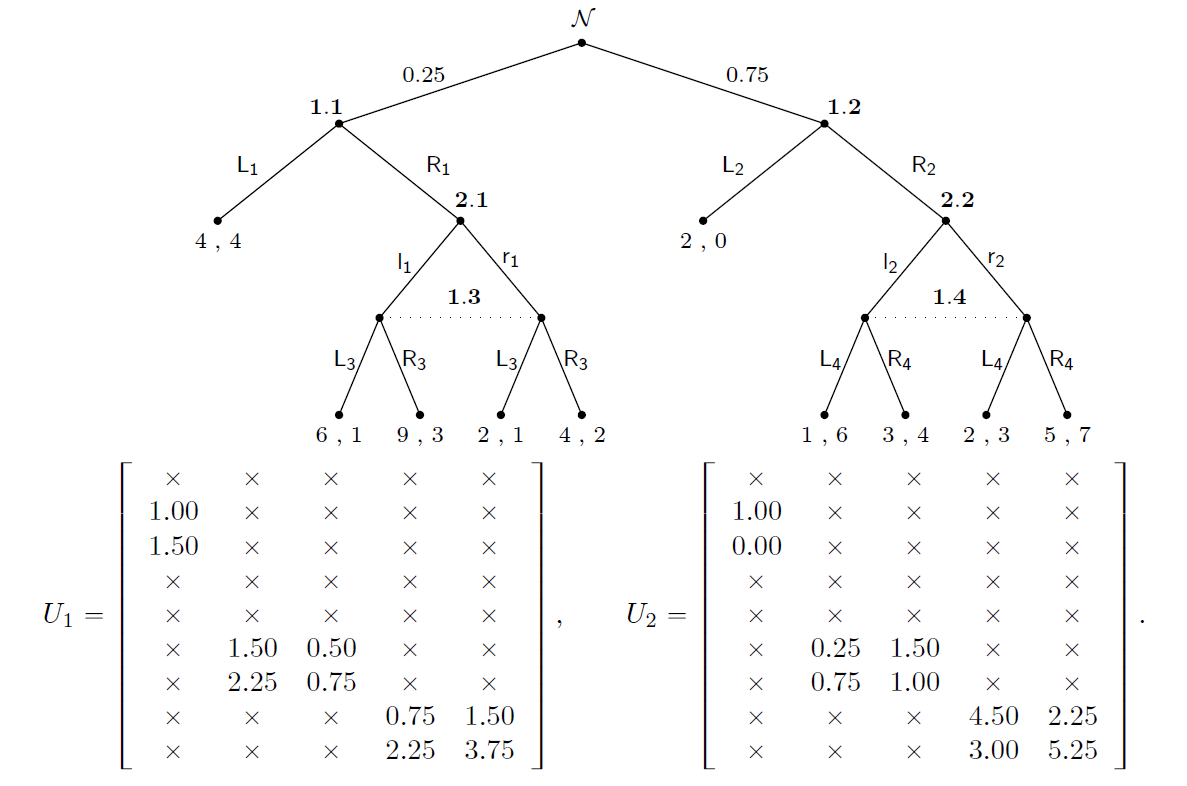
\includegraphics[width=0.9\textwidth]{images/img_1_4_01.png}
\end{figure}
\noindent
Notice that the sequence-form representation has a size, in terms of variables and constraints, that is linear in the size, in terms of terminal nodes, of the game tree.\\\\
\textbf{Exercise 4.0.5} (Expected utility). \textit{Given a game in sequence-form with n players, provide the formula of the
expected utility for a player i.}\\\\
Expected utility $\mathbb{E}_{\mathbf{q} \sim \mathbf{r}}\left[U_{i}(\mathbf{q})\right]$ returns the expected value of the utility of player i given strategy profile $\mathbf{r}$. The formula $\mathbb{E}_{\mathbf{q} \sim \mathbf{r}}\left[U_{i}(\mathbf{q})\right]$ can be written as:
$$
\mathbb{E}_{\mathbf{q} \sim \mathbf{r}}\left[U_{i}(\mathbf{q})\right]=\sum_{q_{1} \in Q_{1}} \sum_{q_{2} \in Q_{2}} \ldots \sum_{q_{n} \in Q_{n}} r_{1}\left(q_{1}\right) r_{2}\left(q_{2}\right) \ldots r_{n}\left(q_{n}\right) U_{i}\left(q_{1}, q_{2}, \ldots, q_{n}\right)
$$
once assigned $U_{i}(\mathbf{q})=0$ for all the profile $\mathbf{q}$ containing at least one non-terminal sequence. The degree of the polynomial is $n$ and, given player $i$, the expected utility is linear in player $i$'s strategy.\\\\

\section{EC 1.5}
\textbf{Exercise 5.0.1} (Kuhn theorem). \textit{Provide the statement of the Kuhn theorem.}\\\\
Given every game with perfect recall and every normal-form strategy, there always exists at least a realization-equivalent agent-form strategy and vice versa.\\\\

\section{EC 1.6}
\textbf{Exercise 6.0.1} (Realization equivalence). \textit{Provide the conditions under which two strategies (even defined over
different representations of the same game) are realization equivalent.}\\\\
(Realization equivalence). Given an extensive-form game, two strategies, even defined on different
representations, are realization equivalent if, for every strategy of the opponents, they induce the same probability
distribution over the outcomes of the game.\\\\
(Sequence/normal-form strategies realization equivalence). Given a game and a player $i$, a sequence-form strategy $r_i$ and a normal-form strategy $\sigma_i$ are realization equivalent if and only if the following property holds for every $q \in Q_i$:
$$ r_{i}(q) = \sum_{p \in P_i:\mathsf{action}(q) \in p} \sigma_{i}(p) $$
The above relation provides a direct way to find a sequence-form strategy given a normal-form strategy. The reverse is more involved, since every sequence-form strategy may be realization equivalent to many normal-form strategies and therefore it is necessary the resolution of a linear equation system.\\\\
(Normal-form strategy derivation from a sequence-form strategy). Given a game and a sequence-form strategy $r_{i}$, the reduced normal-form strategy $\sigma_{i}$ defined as
$$
\sigma_{i}(p)=\prod_{q \in \bar{Q}_{i}: \textsf{action}(q) \in p} r_{i}(q)
$$
for every $p \in P_{i}$, is realization equivalent to $r_{i}^{1}$.\\\\
\textbf{Exercise 6.0.2} (From sequence-form to normal-form). \textit{Given an extensive-form game, its normal-form and sequence-form representations, and a strategy profile defined over the sequence-form, provide a strategy defined over the normal-form that is realization equivalent. Is the latter unique?}\\\\
Consider the following game in extensive form
\begin{figure}[H]
\centering
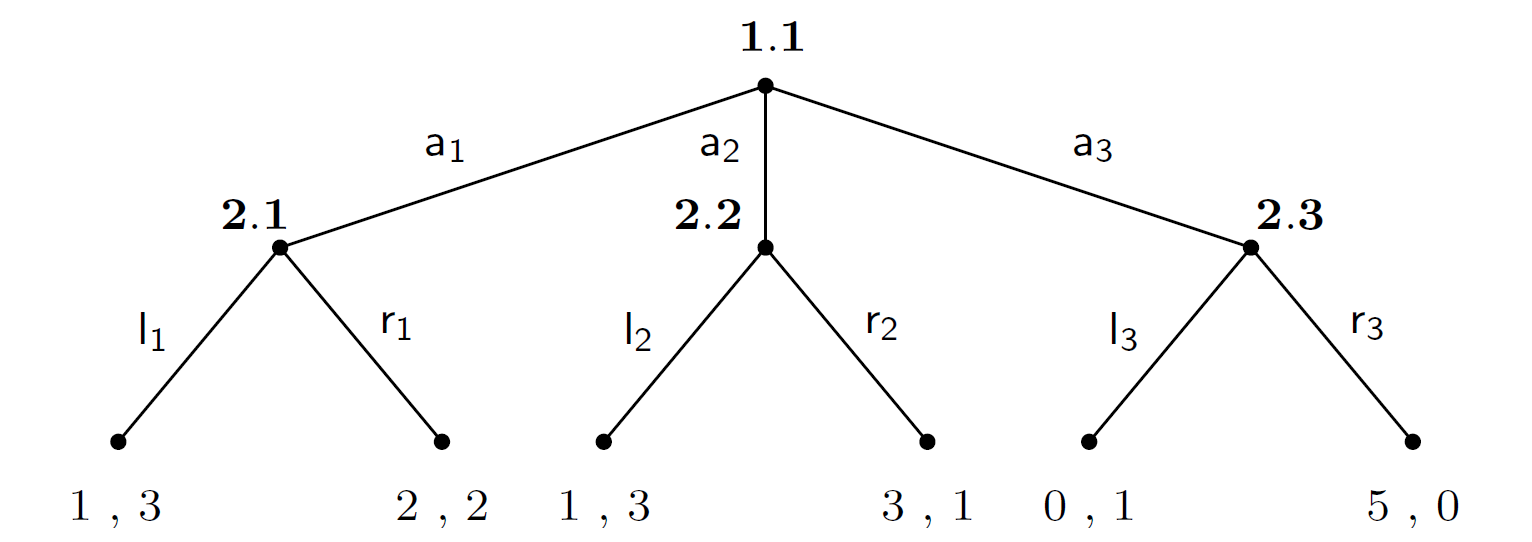
\includegraphics[width=0.6\textwidth]{images/img_1_6_01.png}
\end{figure}
\noindent
its corresponding normal-form representation (the reduced normal form is the same):
\begin{figure}[H]
\centering
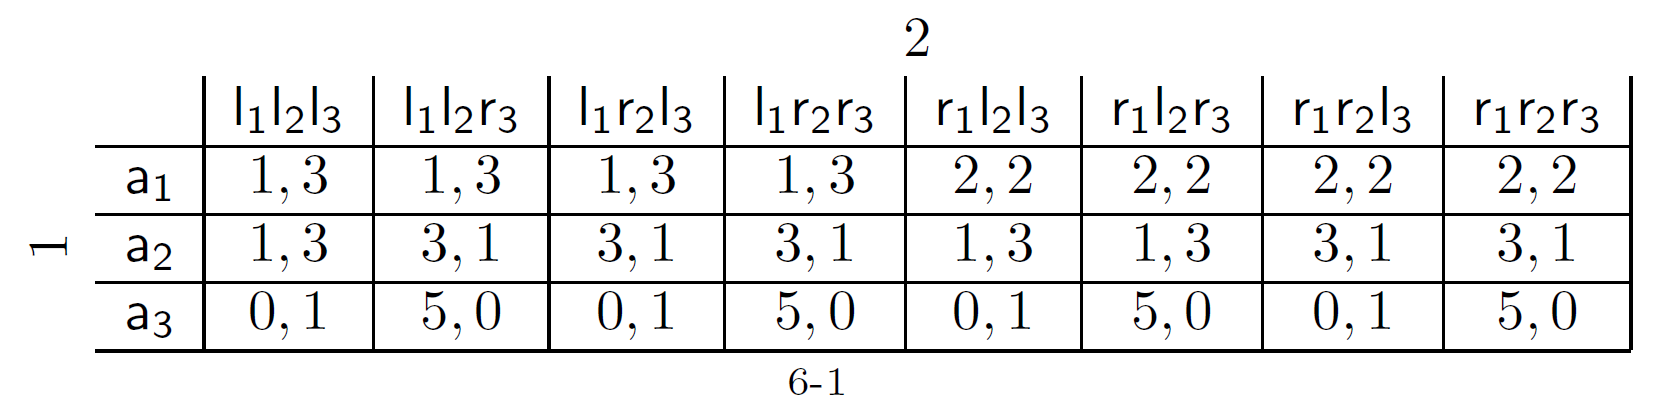
\includegraphics[width=0.6\textwidth]{images/img_1_6_02.png}
\end{figure}
\noindent
and its corresponding sequence-form representation:
\begin{figure}[H]
\centering
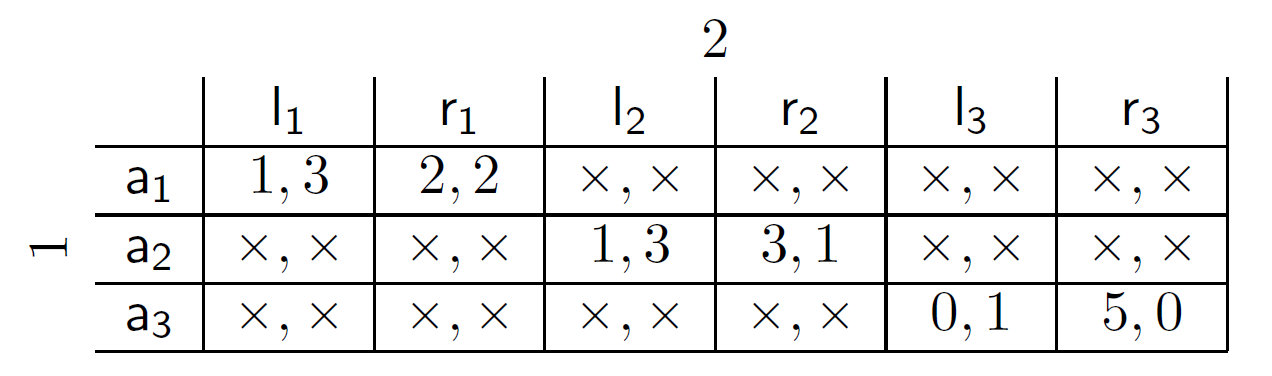
\includegraphics[width=0.6\textwidth]{images/img_1_6_03.png}
\end{figure}
\noindent
(Normal-form strategy derivation from a sequence-form strategy). Consider the following sequence-form strategy:
$$ 
r_{2}=\left[\begin{array}{c}
1.00 \\
0.50 \\
0.50 \\
0.30 \\
0.70 \\
0.25 \\
0.75
\end{array}\right]
$$
In the realization-equivalent strategy $\sigma_{2},$ we have, e.g., plan $p=\mathsf{l}_{1}\mathsf{l}_{2}\mathsf{l}_{3}$ played with probability $\sigma_{2}\left(\mathsf{l}_{1}\mathsf{l}_{2}\mathsf{l}_{3}\right)=0.50 \cdot 0.30 \cdot 0.25$. This derivation does not work for the non-reduced normal form and is not unique.\\\\
\textbf{Exercise 6.0.3} (From normal-form to sequence-form). \textit{Given an extensive-form game, its normal-form and sequence-form representations, and a strategy profile defined over the normal-form, provide a strategy defined over the sequence-form that is realization equivalent. Is the latter unique?}\\\\
(Sequence/normal-form strategies realization equivalence). Consider the example above. Strategies $r_2$ and $\sigma_2$ are realization equivalent if the following equations are satisfied:
$$
\begin{aligned}
&r_{2}\left(\mathrm{l}_{1}\right) & = \ & \sigma_{2}\left(\mathrm{l}_{1} \mathrm{l}_{2} \mathrm{l}_{3}\right) & + \ &  \sigma_{2}\left(\mathrm{l}_{1} \mathrm{l}_{2} \mathrm{r}_{3}\right) & + \ &  \sigma_{2}\left(\mathrm{l}_{1} \mathrm{r}_{2}\mathrm{l}_{3}\right) & + \ &  \sigma_{2}\left(\mathrm{l}_{1} \mathrm{r}_{2} \mathrm{r}_{3}\right)\\
&r_{2}\left(r_{1}\right) & = \ & \sigma_{2}\left(r_{1} l_{2}\mathrm{l}_{3}\right) & + \ &  \sigma_{2}\left(r_{1} l_{2} r_{3}\right) & + \ &  \sigma_{2}\left(r_{1} r_{2}\mathrm{l}_{3}\right) & + \ &  \sigma_{2}\left(r_{1} r_{2} r_{3}\right)\\
&r_{2}\left(\mathrm{l}_{2}\right) & = \ & \sigma_{2}\left(\mathrm{l}_{1}\mathrm{l}_{2}\mathrm{l}_{3}\right) & + \ & \sigma_{2}\left(\mathrm{l}_{1}\mathrm{l}_{2} r_{3}\right) & + \ &  \sigma_{2}\left(r_{1}\mathrm{l}_{2}\mathrm{l}_{3}\right) & + \ &  \sigma_{2}\left(r_{1}\mathrm{l}_{2} r_{3}\right)\\
&r_{2}\left(r_{2}\right) & = \ & \sigma_{2}\left(\mathrm{l}_{1} r_{2}\mathrm{l}_{3}\right) & + \ &  \sigma_{2}\left(\mathrm{l}_{1} r_{2} r_{3}\right) & + \ &  \sigma_{2}\left(r_{1} r_{2}\mathrm{l}_{3}\right) & + \ &  \sigma_{2}\left(r_{1} r_{2} r_{3}\right)\\
&r_{2}\left(\mathrm{l}_{3}\right) & = \ & \sigma_{2}\left(\mathrm{l}_{1} \mathrm{l}_{2}\mathrm{l}_{3}\right) & + \ &  \sigma_{2}\left(\mathrm{r}_{1}\mathrm{l}_{2}\mathrm{l}_{3}\right) & + \ &  \sigma_{2}\left(\mathrm{r}_{1} \mathrm{r}_{2}\mathrm{l}_{3}\right) & + \ &  \sigma_{2}\left(\mathrm{l}_{1} \mathrm{r}_{2}\mathrm{l}_{3}\right)\\
&r_{2}\left(\mathrm{r}_{3}\right) & = \ & \sigma_{2}\left(\mathrm{l}_{1} \mathrm{l}_{2} \mathrm{r}_{3}\right) & + \ &  \sigma_{2}\left(\mathrm{l}_{1} \mathrm{r}_{2} \mathrm{r}_{3}\right) & + \ &  \sigma_{2}\left(\mathrm{r}_{1} \mathrm{r}_{2} \mathrm{r}_{3}\right) & + \ &  \sigma_{2}\left(\mathrm{r}_{1}\mathrm{l}_{2} \mathrm{r}_{3}\right)
\end{aligned}
$$
Notice that $ r_{2}(q) = \frac{1}{2} $ for every $q$ is realization equivalent to $ \sigma_{2}(p) = \frac{1}{8} $ for every $p$, but it is realization equivalent also to $ \sigma_{2}(l_{1} l_{2} l_{3}) = \sigma_{2}(r_{1} r_{2} r_{3}) = \frac{1}{2} $ and $ \sigma_{2}(p) = 0 $ for all the other $p$. The derivation is unique.\\\\
\textbf{Exercise 6.0.4} (Sequence-form and reduced normal-form). \textit{What is the relation between sequence-form representation and reduced normal-form representation?}\\\\
(Sequence/reduced-normal-form strategies realization equivalence). Every pure sequence-form strategy corresponds to a single plan in the reduced normal form.\\\\
The observation above shows that the number of pure realization plans is exponentially large in the size of the game tree, the number of plans of the reduced normal-form being exponentially large. When using the reduced normal-form representation, we have a direct way to derive a strategy that is realization equivalent to a given realization plan.\\\\

\section{EC 1.7}
\textbf{Exercise 7.0.1} (Zero-sum/constant-sum/strictly competitive games). \textit{Provide the definition of:
\begin{itemize}
\item 2-player zero-sum game;
\item 2-player constant-sum game;
\item 2-player strictly-competitive game.
\end{itemize}
Furthermore, describe their relationships, and their properties in the players utility space.}\\\\
(Zero-sum game). A zero-sum game is a game in which, for each terminal node $ w $ in the game tree (i.e., each outcome), the following property holds: $ \sum_{i \in N} U_{i}(w) = 0 $.\\\\
(Zero-sum game and utility space). Given the space of players' utilities $ (U_{1}, U_{2}, \allowbreak \ldots, U_{n}) $ in $ \mathbb{R}^n $,
each terminal node can be mapped as a point in such a space and, in a zero-sum game, all these points lie on a hyperplane $ \sum_{i \in N} U_{i} = 0 $.\\\\
(Constant-sum game). A constant-sum game is a game in which, for each terminal node $ w $ in the game tree (i.e., each outcome), the following property holds: $ \sum_{i \in N} U_{i}(w) = constant $.\\\\
(Constant-sum game and utility space). Given the space of players’ utilities $ (U_{1}, U_{2}, \ldots, U_{n}) $ in $ \mathbb{R}^n $, each terminal node can be mapped as a point in such a space and, in a constant-sum game, all these
points lie on a hyperplane $ \sum_{i \in N} U_{i} = constant $.\\\\
(Strictly competitive game). A strictly competitive game is a 2 -player game in which, for any pair of strategy profiles $ \sigma, \sigma^{\prime}, \mathbb{E}_{\mathbf{a} \sim \sigma} [ U_{1}(\mathbf{a}) ] < \mathbb{E}_{\mathbf{a} \sim \sigma^{\prime}} [ U_{1}(\mathbf{a}) ] $ if and only if $ \mathbb{E}_{\mathbf{a} \sim \sigma} [ U_{2}(\mathbf{a}) ] > \mathbb{E}_{\mathbf{a} \sim \sigma^{\prime}} [ U_{2}(\mathbf{a}) ] $.\\
Strictly-competitive games capture the situation in which, for every given strategy profile and for any perturbation of it, a player increases her expected utility if and only if the opponent reduces her expected utility. It is known that a strictly-competitive game is just a zero-sum game once an affine transformation is applied.\\\\
(Strictly competitive game and utility space). Given the space of players’ utilities $ (U_1,U_2) $ in $ \mathbb{R}^2 $, each terminal node can be mapped as a point in such a space and, in a strictly competitive game, all these points lie on a hyperplane $ \sum_{i \in N} \alpha_{i} U_{i} = constant $, where $ \alpha_{i} \in (0, 1] $.\\\\
(Constant-sum game as zero-sum game). A constant-sum game is equivalent to a zero-sum game, once the constant has been subtracted from the utility of a player.\\\\
(Strictly competitive and zero-sum games). Any strictly-competitive game is equivalent to a zero-sum game once an affine transformation, in principle different for each player, is applied.\\\\
\textbf{Exercise 7.0.2} (Polymatrix games). \textit{Provide the definition of Polymatrix games and the formula of players expected utility. Furthermore, provide the conditions under which a Polymatrix game is zero sum.}\\\\
A Polymatrix game in normal-form representation is a tuple $ (N, A, U) $ where:
\begin{itemize}
\item the definitions of $ N $ and $ A $ are standard as in normal-form games;
\item $ U = \{ U_{1}, U_{2}, \ldots, U_{n} \} $ and each utility function $ U_{i} $ is defined as\\
$ \sum_{j \in N \backslash\{i\}} U_{i, j} $ where each $ U_{i, j} $ is defined as $ U_{i, j}: A_{i} \times A_{j} \rightarrow \mathbb{R} $ and therefore each $ U_{i, j} $ can be described as a matrix.
\end{itemize}
(Polymatrix game and expected utility). The formula $ \mathbb{E}_{\mathbf{a} \sim \mathbf{s}} [U_{i}(\mathbf{a})] $ in a Polymatrix game can be written as:
$$
\mathbb{E}_{\mathbf{a} \sim \sigma} [U_{i}(\mathbf{a}) ] = \sum_{j \in N \backslash\{i\}} \sum_{a_{i} \in A_{i}} \sum_{a_{j} \in A_{j}} \sigma_{i} (a_{i}) \sigma_{j} (a_{j}) U_{i, j} (a_{i}, a_{j})
$$
The degree of the polynomial is 2 (independently from n) and, given player i, the expected utility is linear
in player $ i $’s strategy.\\\\
(Zero-sum Polymatrix games). A Polymatrix game with players $ N $ is zero sum if for every $ a \in A_1 \times A_2 \times \ldots \times A_n $ we have $ \sum_{i \in N} U_{i}(a) = 0 $.\\\\
(Zero-sum and zero-sum pairwise Polymatrix games). Any zero-sum Polymatrix game is equivalent to a Polymatrix game where $ U_{i,j} + U_{i,j}^T = 0 $. These last games are called zero-sum pairwise Polymatrix
games.


\section{EC 1.8}
\textbf{Exercise 8.0.1} (Bayesian games). \textit{Given a Bayesian game in epistemic-form, provide the representation in extensive-form.}\\\\
A simultaneous-moves Bayesian game in epistemic-form representation is a tuple $(N, A, \Theta, \Omega, U)$ where:
\begin{itemize}
\item $ N = \{ 1, 2, \ldots, n \} $ is the set of players;
\item $ A = \{ A_{1}, A_{2}, \ldots, A_{n} \} $ is the set of the actions of all the players and $ A_{i} = \{ a_{1}, a_{2}, \ldots, a_{m_{i}} \} $ is the set of player $ i $'s actions;
\item $ \Theta = \Theta_{1} \times \Theta_{2} \times \ldots \times \Theta_{n} $ is the set of the types of all the players and $ \Theta_{i} = \{ \theta_{i, 1}, \theta_{i, 2}, \ldots, \theta_{i, k_{i}} \} $ is the set of the types of player $ i $
\item $ \Omega: \Theta \rightarrow \Delta(\Theta) $ returns the probability associated with each $ ( \theta_{1}, \theta_{2}, \ldots, \theta_{n} ) $ where $ \theta_{i} \in \Theta_{i} $
\item $ U= \{U_{1}, U_{2}, \ldots, U_{n} \} $ is the set of the utility functions of all the players and $ U_{i}: A_{1} \times A_{2} \times \ldots \times A_{n} \times \Theta \rightarrow \mathbb{R} $ is the utility function of player $ i $.
\end{itemize}
\noindent
Epistemic-form:\\
(Bayesian Battle of sexes). Consider a Bayesian game composed of:
\begin{itemize}
\item $ N = \{ 1, 2 \} $
\item $ A = \{A_{1}, A_{2} \} $ with $ A_{1} = \{ \mathrm{B}, \mathrm{S} \}, A_{2} = \{ \mathrm{B}, \mathrm{S} \} $
\item $ \Theta = \{ \Theta_{1}, \Theta_{2} \} $ with $ \Theta_{1} = \{ \theta_{1,1}, \theta_{1,2} \}, \Theta_{2} = \{ \theta_{2,1}, \theta_{2,2} \} $
\item $ \Omega= \{ \Omega_{1}, \Omega_{2} \} $ with:
$$
\qquad \Omega_{1}= \{ \begin{array}{ll}
									0.2 & \theta_{1.1} \\
									0.8 & \theta_{1.2}
					  \end{array}, 
\quad \Omega_{2} = \{ \begin{array}{ll}
									0.3 & \theta_{2.1} \\
									0.7 & \theta_{2.2}
					  \end{array}
$$
\item utility functions are represented by means of the following bi-matrices:
\end{itemize}
\begin{figure}[H]
\centering
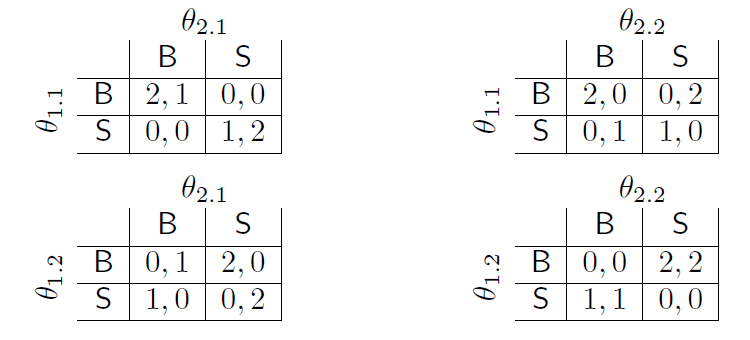
\includegraphics[width=0.7\textwidth]{images/img_1_8_01.png}
\end{figure}
Extensive-form:
\begin{figure}[H]
\centering
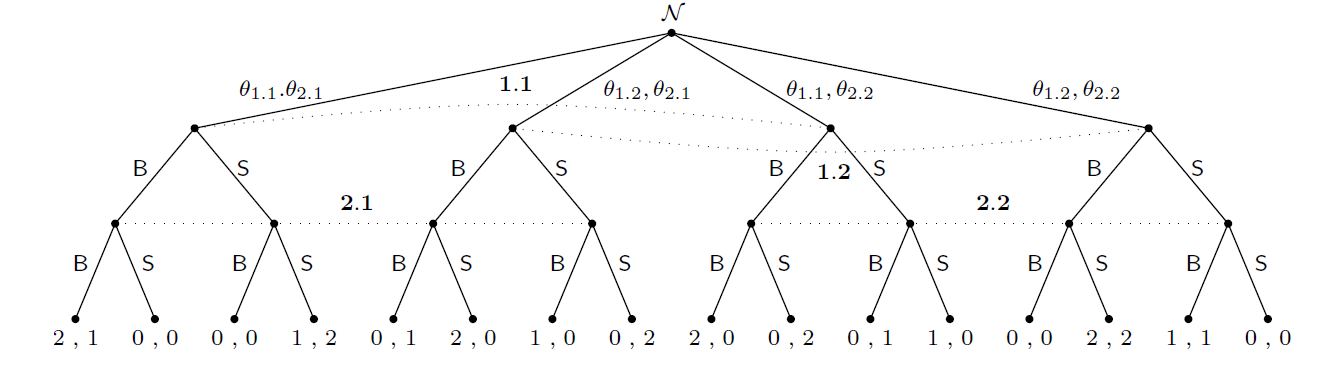
\includegraphics[width=\textwidth]{images/img_1_8_02.png}
\end{figure}



